\documentclass[crop,tikz]{standalone}

% helper tool: www.mathcha.io

\usetikzlibrary{arrows.meta}

\begin{document}

% set font to serif roman
\rmfamily

\tikzset{every picture/.style={line width=0.75pt}} %set default line width to 0.75pt      

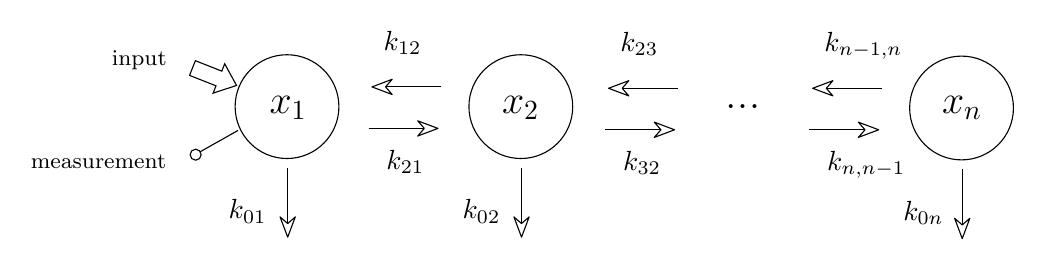
\begin{tikzpicture}[x=0.75pt,y=0.75pt,yscale=-1,xscale=1]
%uncomment if require: \path (0,108); %set diagram left start at 0, and has height of 108

%Shape: Circle [id:dp9820664449106131] 
\draw   (100.68,40.17) .. controls (100.68,26.36) and (111.87,15.17) .. (125.68,15.17) .. controls (139.49,15.17) and (150.68,26.36) .. (150.68,40.17) .. controls (150.68,53.97) and (139.49,65.17) .. (125.68,65.17) .. controls (111.87,65.17) and (100.68,53.97) .. (100.68,40.17) -- cycle ;
%Straight Lines [id:da4959810469294802] 
\draw [-{Stealth[length=3mm, open, round]}]    (126.01,69.67) -- (126.01,103.33) ;
%\draw [shift={(126.01,105.33)}, rotate = 270] [color={rgb, 255:red, 0; green, 0; blue, 0 }  ][line width=0.75]    (10.93,-3.29) .. controls (6.95,-1.4) and (3.31,-0.3) .. (0,0) .. controls (3.31,0.3) and (6.95,1.4) .. (10.93,3.29)   ;
%Straight Lines [id:da22208007705967803] 
\draw    (83.76,61.97) -- (102.09,51.64) ;
%Shape: Circle [id:dp2351936246373434] 
\draw   (79,63.33) .. controls (79,61.86) and (80.19,60.67) .. (81.66,60.67) .. controls (83.12,60.67) and (84.31,61.86) .. (84.31,63.33) .. controls (84.31,64.8) and (83.12,65.98) .. (81.66,65.98) .. controls (80.19,65.98) and (79,64.8) .. (79,63.33) -- cycle ;
%Right Arrow [id:dp7195375552934989] 
\draw   (81.53,18.04) -- (94.27,23.07) -- (95.66,19.53) -- (101.36,29.96) -- (90.07,33.69) -- (91.47,30.15) -- (78.73,25.12) -- cycle ;
%Straight Lines [id:da7788757647947052] 
\draw [-{Stealth[length=3mm, open, round]}]    (200,30.67) -- (166.33,30.67) ;
%\draw [shift={(164.33,30.67)}, rotate = 360] [color={rgb, 255:red, 0; green, 0; blue, 0 }  ][line width=0.75]    (10.93,-3.29) .. controls (6.95,-1.4) and (3.31,-0.3) .. (0,0) .. controls (3.31,0.3) and (6.95,1.4) .. (10.93,3.29)   ;
%Straight Lines [id:da7932076941820535] 
\draw [-{Stealth[length=3mm, open, round]}]    (165,50.67) -- (198.67,50.67) ;
%\draw [shift={(200.67,50.67)}, rotate = 180] [color={rgb, 255:red, 0; green, 0; blue, 0 }  ][line width=0.75]    (10.93,-3.29) .. controls (6.95,-1.4) and (3.31,-0.3) .. (0,0) .. controls (3.31,0.3) and (6.95,1.4) .. (10.93,3.29)   ;
%Shape: Circle [id:dp5937484282010274] 
\draw   (213.33,40.17) .. controls (213.33,26.36) and (224.53,15.17) .. (238.33,15.17) .. controls (252.14,15.17) and (263.33,26.36) .. (263.33,40.17) .. controls (263.33,53.97) and (252.14,65.17) .. (238.33,65.17) .. controls (224.53,65.17) and (213.33,53.97) .. (213.33,40.17) -- cycle ;
%Straight Lines [id:da48255207978324854] 
\draw [-{Stealth[length=3mm, open, round]}]    (238.67,69.67) -- (238.67,103.33) ;
%\draw [shift={(238.67,105.33)}, rotate = 270] [color={rgb, 255:red, 0; green, 0; blue, 0 }  ][line width=0.75]    (10.93,-3.29) .. controls (6.95,-1.4) and (3.31,-0.3) .. (0,0) .. controls (3.31,0.3) and (6.95,1.4) .. (10.93,3.29)   ;
%Straight Lines [id:da6046640888454475] 
\draw [-{Stealth[length=3mm, open, round]}]    (314,31.33) -- (280.33,31.33) ;
%\draw [shift={(278.33,31.33)}, rotate = 360] [color={rgb, 255:red, 0; green, 0; blue, 0 }  ][line width=0.75]    (10.93,-3.29) .. controls (6.95,-1.4) and (3.31,-0.3) .. (0,0) .. controls (3.31,0.3) and (6.95,1.4) .. (10.93,3.29)   ;
%Straight Lines [id:da5100366191108595] 
\draw [-{Stealth[length=3mm, open, round]}]    (279,51.33) -- (312.67,51.33) ;
%\draw [shift={(314.67,51.33)}, rotate = 180] [color={rgb, 255:red, 0; green, 0; blue, 0 }  ][line width=0.75]    (10.93,-3.29) .. controls (6.95,-1.4) and (3.31,-0.3) .. (0,0) .. controls (3.31,0.3) and (6.95,1.4) .. (10.93,3.29)   ;
%Straight Lines [id:da2623286526527041] 
\draw [-{Stealth[length=3mm, open, round]}]    (412.33,31.33) -- (378.67,31.33) ;
%\draw [shift={(376.67,31.33)}, rotate = 360] [color={rgb, 255:red, 0; green, 0; blue, 0 }  ][line width=0.75]    (10.93,-3.29) .. controls (6.95,-1.4) and (3.31,-0.3) .. (0,0) .. controls (3.31,0.3) and (6.95,1.4) .. (10.93,3.29)   ;
%Straight Lines [id:da24531280456249516] 
\draw [-{Stealth[length=3mm, open, round]}]    (377.33,51.33) -- (411,51.33) ;
%\draw [shift={(413,51.33)}, rotate = 180] [color={rgb, 255:red, 0; green, 0; blue, 0 }  ][line width=0.75]    (10.93,-3.29) .. controls (6.95,-1.4) and (3.31,-0.3) .. (0,0) .. controls (3.31,0.3) and (6.95,1.4) .. (10.93,3.29)   ;
%Shape: Circle [id:dp23694417720919403] 
\draw   (425.67,40.83) .. controls (425.67,27.03) and (436.86,15.83) .. (450.67,15.83) .. controls (464.47,15.83) and (475.67,27.03) .. (475.67,40.83) .. controls (475.67,54.64) and (464.47,65.83) .. (450.67,65.83) .. controls (436.86,65.83) and (425.67,54.64) .. (425.67,40.83) -- cycle ;
%Straight Lines [id:da5346189238124088] 
\draw [-{Stealth[length=3mm, open, round]}]    (451,70.33) -- (451,104) ;
%\draw [shift={(451,106)}, rotate = 270] [color={rgb, 255:red, 0; green, 0; blue, 0 }  ][line width=0.75]    (10.93,-3.29) .. controls (6.95,-1.4) and (3.31,-0.3) .. (0,0) .. controls (3.31,0.3) and (6.95,1.4) .. (10.93,3.29)   ;

% Text Node
\draw (116,34) node [anchor=north west][inner sep=0.75pt]  [font=\Large]  {$x_{1}$};
% Text Node
\draw (96.34,83.73) node [anchor=north west][inner sep=0.75pt]    {$k_{01}$};
% Text Node
\draw (40,12) node [anchor=north west][inner sep=0.75pt]   [align=left] {{\footnotesize input}};
% Text Node
\draw (1,62) node [anchor=north west][inner sep=0.75pt]   [align=left] {{\footnotesize measurement}};
% Text Node
\draw (172.34,59.73) node [anchor=north west][inner sep=0.75pt]    {$k_{21}$};
% Text Node
\draw (228,34) node [anchor=north west][inner sep=0.75pt]  [font=\Large]  {$x_{2}$};
% Text Node
\draw (209,83.73) node [anchor=north west][inner sep=0.75pt]    {$k_{02}$};
% Text Node
\draw (171.01,2.4) node [anchor=north west][inner sep=0.75pt]    {$k_{12}$};
% Text Node
\draw (286.34,60.4) node [anchor=north west][inner sep=0.75pt]    {$k_{32}$};
% Text Node
\draw (285.01,3.07) node [anchor=north west][inner sep=0.75pt]    {$k_{23}$};
% Text Node
\draw (335.33,38) node [anchor=north west][inner sep=0.75pt]  [font=\LARGE] [align=left] {...};
% Text Node
\draw (384.68,60.4) node [anchor=north west][inner sep=0.75pt]    {$k_{n,n-1}$};
% Text Node
\draw (440,34) node [anchor=north west][inner sep=0.75pt]  [font=\Large]  {$x_{n}$};
% Text Node
\draw (421.33,84.4) node [anchor=north west][inner sep=0.75pt]    {$k_{0n}$};
% Text Node
\draw (383.34,3.07) node [anchor=north west][inner sep=0.75pt]    {$k_{n-1,n}$};

\end{tikzpicture}

\end{document}